\chapter{Capability Table and Capability Management}\label{ch:capability-table-management}

\section{The Concept of Capability}\label{sec:2-capability-concept}

A capability (Capability) is a kind of credential used to control access permissions that was first introduced in multi-user computer systems\hyperref[cite:2-1]{{[}1{]}}. It is an unforgeable credential that uniquely identifies a certain resource as well as the operations that are permitted on that resource. For example, a Unix file descriptor is a kind of capability\hyperref[cite:2-2]{{[}2{]}}; a Windows access permission is also a kind of capability. In a sense, a capability is a fat
pointer (Fat Pointer) to a certain resource.

We use the following three principles to guarantee the security of the system\hyperref[cite:2-2]{{[}2{]}}:

\begin{enumerate}
\def\labelenumi{\arabic{enumi}.}
\item
  Capabilities cannot be forged and cannot be arbitrarily modified in user mode;
\item
  A process can only obtain capabilities through well-defined authorization interfaces;
\item
  Capabilities are only given to those processes that are responsible for managing the resource at system design time.

  Third-generation microkernels generally adopt the concept of capabilities to manage resources. In RME, all kernel resources are managed using capabilities, and all capabilities reside in capability tables in kernel space. Each process corresponds to one capability table (Capability
  Table), and when a system call is invoked, the system looks up kernel objects from that process's capability table. Each capability has a series of operation flag bits; if a certain capability possesses a certain operation flag bit, then that operation can be performed on the kernel object through this capability\hyperref[cite:2-3]{{[}3{]}}. The vast majority of systems, such as seL4\hyperref[cite:2-5]{{[}5{]}}, have operation flag bits. However, for some other systems\footnote{such as Composite}, a certain kernel object has only one operation, so a separate operation flag bit is not needed\hyperref[cite:2-4]{{[}4{]}}.

  Besides capabilities, there is another method called the access control list (Access Control List, ACL)\hyperref[cite:2-6]{{[}6{]}}. It can also be used to manage permissions, but its access permission management granularity is relatively coarse, and the table easily becomes very large. Its advantage is that granting and revoking permissions is relatively simple\footnote{especially the revocation operation}.

  In RME, using the concept of capabilities, discretionary access control (Discretionary Access
  Control, DAC) and mandatory access control (Mandatory Access
  Control, MAC) can be readily implemented, multi-level security mechanisms can also be readily built, and the design of the whole user application can be planned according to the principle of least privilege.
\end{enumerate}

\section{Capability Table Operations and Capability States}\label{sec:2-capability-table-operations-and-states}

A capability table is a kernel object used to store capabilities. In RME it is a linear array, and the size of each array position is a fixed 8 machine words, which can be used to store one capability. Inside a capability are recorded the exact type of the kernel resource, its exact location in kernel memory\footnote{a pointer into the kernel address space}, the parent capability of the capability, the capability delegation reference count, and the current state of the capability. In addition, there is a timestamp counter used to guarantee the quiescence (Quiescence) of capability operations under multi-core parallelism.

\subsection{Capability Types}\label{subsec:2-capability-types}

In RME, there are altogether 8 types of capabilities\footnote{excluding the empty capability}, as shown in the table below. For information about capabilities of the corresponding types, please consult the corresponding chapters for reference. This chapter only describes the content related to capability table capabilities.

\begin{xltabular}{\textwidth}{@{}>{\hsize=0.8412\hsize\raggedright\arraybackslash}X>{\hsize=0.7467\hsize\raggedright\arraybackslash}X>{\hsize=1.4121\hsize\raggedright\arraybackslash}X@{}}
\caption{Types of Capabilities}\label{tab:2-1-capability-types}\\
\toprule
Capability type number & Capability type & Purpose\tabularnewline
\endfirsthead
\toprule
Capability type number & Capability type & Purpose\tabularnewline
\midrule
\endhead
\bottomrule
\endlastfoot
RME\_CAP\_TYPE\_NOP & Empty capability &
This position of the capability table is an empty capability.\tabularnewline
RME\_CAP\_TYPE\_KFN & Kernel function capability &
The capability required to invoke special-function kernel functions.\tabularnewline
RME\_CAP\_TYPE\_KOM & Kernel memory capability &
The capability required to create kernel objects using a region of kernel memory.\tabularnewline
RME\_CAP\_TYPE\_CPT & Capability table capability &
Points to a capability table object; can be used for capability table management.\tabularnewline
RME\_CAP\_TYPE\_PGT & Page directory capability &
Points to a page directory object; can be used for memory management.\tabularnewline
RME\_CAP\_TYPE\_PRC & Process capability &
Points to a process object; can be used for process management.\tabularnewline
RME\_CAP\_TYPE\_THD & Thread capability &
Points to a thread object; can be used for thread management.\tabularnewline
RME\_CAP\_TYPE\_INV & Invocation capability &
Points to an invocation object; can be used for synchronous invocation.\tabularnewline
RME\_CAP\_TYPE\_SIG & Signal endpoint capability &
Points to a signal endpoint object; can send and receive signals.\tabularnewline
\end{xltabular}
\nopagebreak[4]

Each kind of capability represents the power to perform operations on that kind of kernel object, and also represents the functionality that the kernel object can implement. It is worth noting that a capability pointing to a capability table\footnote{abbreviated as capability table capability} is a meta-capability of the system, because this capability has the power to modify the capability table and can determine the contents of the capability table.

\subsection{Capability Delegation Reference Count and Parent Capability}\label{subsec:2-reference-count-and-parent-capability}

For those capabilities created in the process of creating kernel objects, we call them root capabilities; for those capabilities created by the capability delegation operation, we call them leaf capabilities. The mark of a root capability is that its attached attribute is set to ROOT, while the pointer used to record the root capability instead records the reference count, which is 0 at initial creation.

The delegation reference count and the root capability of a capability are used to track capability delegation relationships. A capability can be delegated from one capability table to another capability table; in this case we call the source capability the parent capability and the destination capability the child capability. The root capability pointer of the child capability must point to the root capability, and at the same time the reference count of the root capability must be incremented by 1. That is, if the parent capability is a root capability, then the root capability pointer of the child capability points to the parent capability; if the parent capability is a leaf capability, then the root capability pointer of the child capability equals the root capability pointer of the parent capability. It is worth noting that some kernel objects also increment the reference count when they reference each other.

When removing capabilities, it is required that the leaf capabilities and all references to the kernel object be removed first, and only then can the root capability be deleted.\hyperref[cite:2-4]{{[}4{]}}

\subsection{Capability States}\label{subsec:2-capability-states}

A capability has four states: empty, creating, valid, and frozen. These four states can be converted into each other through system calls.

To create a capability, invoke the corresponding kernel object creation function, use a capability table capability to designate the capability table being operated on\footnote{Since the creation operation needs to add a capability into the capability table and thus modifies the capability table, a capability table capability is required; similarly, destroying a kernel object also requires a capability table capability.}, and designate the kernel virtual memory address of the kernel object to be created as well as some necessary parameters. At this point, the empty slot of the designated capability table is first changed to ``creating'' by an atomic compare-and-swap instruction; once creation succeeds, the state is changed to ``valid''; otherwise it remains ``empty'' and the corresponding error code is returned. When creating a capability, if kernel memory needs to be allocated, then a kernel memory capability is also required. For kernel memory capabilities, please refer to the description in the next chapter.

There are two implementations for capability reclamation. One implementation is that of systems such as seL4 and Fiasco.OC, which support operating-system-level capability reclamation operations; that is, they only support the deletion operation, and during deletion they recursively traverse the entire capability delegation tree to reclaim all capabilities that were delegated. The RME system adopts the other implementation, which splits capability removal and deletion into two operations. The operating system does not perform the work of recursive traversal reclamation; this work must be done by the user mode. The benefit of doing so is that no kernel preemption points need to be introduced, but the drawback is that the user must track every capability delegation and take responsibility for capability reclamation themselves.\hyperref[cite:2-4]{{[}4{]}}

To delete or remove a capability, the position must first be frozen. The freezing operation is performed through the capability freezing system call. At this point, the valid bit of the designated capability table is changed to ``frozen''. If freezing does not succeed, then the corresponding error code is returned. If freezing succeeds, then after the capability operation reaches quiescence, the function can be invoked to delete/remove it. Among these, the deletion operation deletes the corresponding kernel object itself while removing the capability; removal, however, only removes the capability without deleting the kernel object. After a capability is removed, it returns to the ``empty'' state. For leaf capabilities, only the capability removal operation can be used; for root capabilities, only the deletion operation corresponding to that kernel object can be used.

The deletion operation and the removal operation also have subtle behavioral differences. If the deletion operation detects that the kernel object cannot be deleted because references to it still exist, then it unfreezes the root capability and returns RME\_ERR\_CPT\_REFCNT to make it convenient for the user to continue operating. If the user needs to delete, then the root capability must be frozen again before deletion. When the deletion operation detects that deletion is impossible for other reasons, it does not perform the unfreeze operation. Because the removal operation does not check references to the kernel object, it will not unfreeze the leaf capability even if the operation cannot proceed.

\subsection{Timestamp Counter and Multi-Core Parallelism Considerations}\label{subsec:2-timestamp-counter-and-multicore-parallelism}

Execution flows in a multi-core environment are very complex. There are some kernel data structures that are not expected to be modified simultaneously in such complex operations; they require all operations to be atomic. Therefore, there are two solutions: the first solution is to take a lock for every operation, and the second solution is to use atomic operations when changing capability states. The locking approach introduces extra operations, is slower, and also causes cache line contention. Cache line contention refers to CPU1 attempting to modify the cache line while CPU2 attempts to query the state of that cache line, which causes CPU2's cache to be invalidated frequently; this is equivalent to greatly reducing the memory access speed and causes the efficiency of frequent capability operations to drop severely. The atomic operation approach has fewer of these problems, but brings extra implementation difficulty. In RME, we adopt the latter approach to achieve multi-core parallelism.

The RME kernel uses a large number of read-modify-write operations composed of compare-and-swap atomic operations and atomic increment operations to modify capabilities. The kernel also uses a timestamp counter to ensure that there are no conflicts between kernel operations, such as a kernel object being used on one CPU being deleted on another CPU.

If we want to delete or remove a capability, we must ensure that the capability has already been frozen for a period of time. We call this period the capability quiescence period. The length of this period can be configured in the kernel. It is required to be configured to be at least longer than twice the kernel's worst-case execution time. In this way, we can ensure that when the capability is deleted or removed, the capability has already settled down; that is, all operations involving this capability on all CPU cores have already completed, so there will be no mutually conflicting operations. For example, CPU1 is trying to delete capability A, while CPU2 simultaneously tries to use it. CPU2 may have already completed the validity check of the operation and be in the middle of performing that operation; if CPU1 deletes the capability directly without freezing, it may affect the execution of CPU2's corresponding operation. The timestamp counter inside each capability exists precisely to record the freeze time. It records the time at which the last freezing operation began, ensuring that no removal or deletion operation begins before the capability is completely frozen.

The complete capability state transition diagram is shown below. When creation begins, the CPU performing the creation performs a compare-and-swap operation on the empty slot, marking the start of creation; the slot is occupied until creation is complete, at which point the slot is marked as valid, and the capability can be used from then on; if the capability is not referenced and one wants to destroy it after use, then it must first be frozen. A newly created capability must wait for a quiescence period before it can be frozen, and a frozen capability must wait for a quiescence period before it can be removed or deleted.

When deleting or removing a capability, we must first complete all checks and confirm that the capability can be deleted or removed; afterwards, we change the state of the current slot to empty through a compare-and-swap atomic operation to guarantee that only the operation on one CPU core can proceed; finally we perform the real subsequent operations, namely kernel object destruction (deletion) or root capability dereferencing (removal). In RME, after the deletion or removal operation is complete, a new creation operation can begin immediately. The reason is that RME has already saved the information required for subsequent operations into local variables before modifying the slot state; after the modification it no longer accesses that capability slot, but instead uses the saved information to perform the subsequent operations. In Composite\hyperref[cite:2-4]{{[}4{]}}, the information in that slot may still be used in subsequent processing after the modification, so a quiescence period must also be inserted here to prevent this position from being overwritten by a newly created capability.

\begin{figure}[htbp]
    \centering
    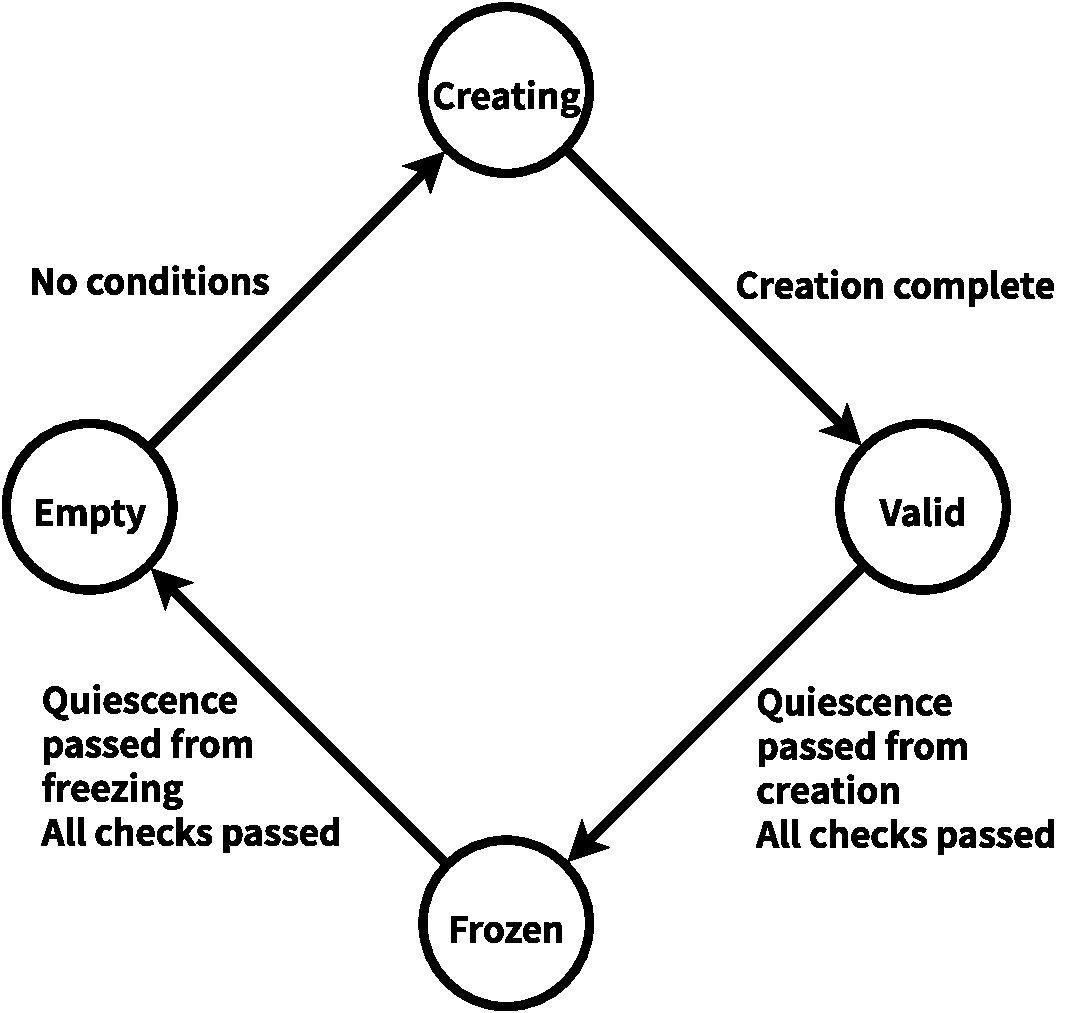
\includegraphics[width=0.72\textwidth]{Figure/image5.pdf}
    \caption{Life Cycle of Capabilities}
    \label{fig:2-1-capability-lifecycle}
\end{figure}

\needspace{16\baselineskip}
The reason why the quiescence period is required to be at least twice the kernel's worst-case execution time is as follows: when invoking the capability freezing operation, we first update the capability's timestamp, and then mark the capability as frozen through an atomic operation. Therefore we have the following timeline:

\begin{figure}[htbp]
    \centering
    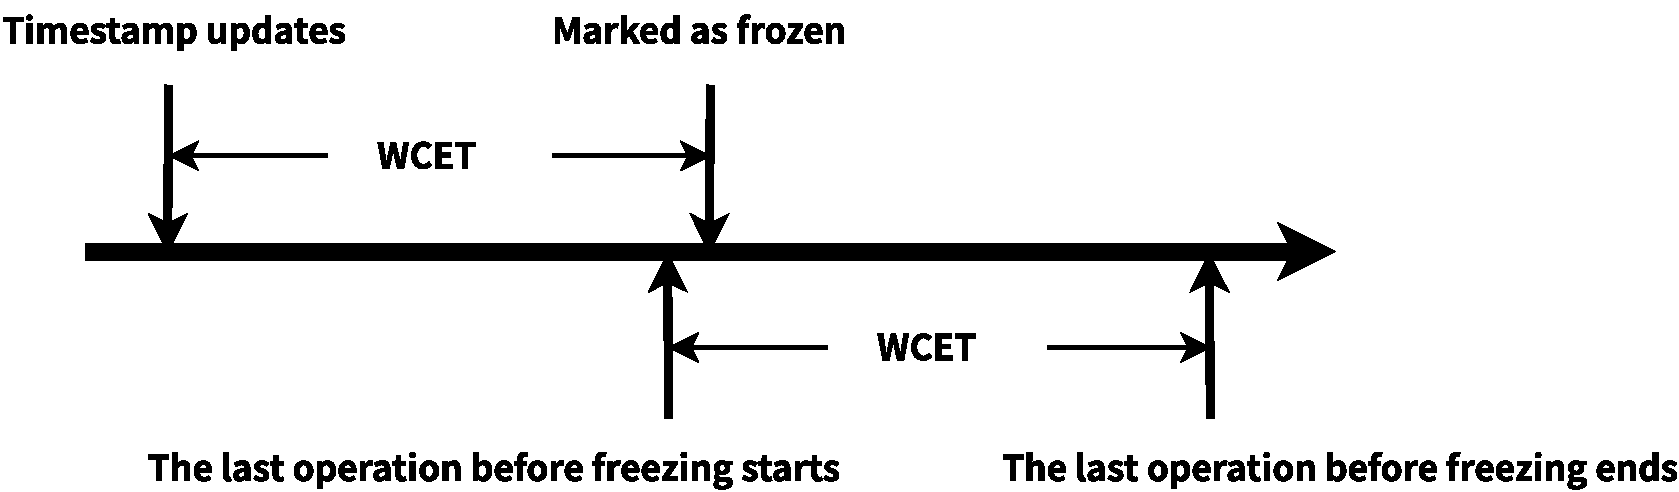
\includegraphics[width=0.72\textwidth]{Figure/image6.pdf}
    \caption{Timeline of Capability Freezing}
    \label{fig:2-2-capability-freeze-timeline}
\end{figure}

It can be seen from this timeline that at most two kernel worst-case execution times may elapse from updating the timestamp to the end of the last operation before freezing. In practical use, it is recommended to configure the quiescence period to at least 20 times the kernel's worst-case execution time\footnote{one order of magnitude higher is recommended}, because in engineering the estimation of the worst-case execution time is often accurate only in order of magnitude.

The principle explained above is the same for the creation------freezing quiescence period of capabilities, and is not repeated here.

\subsection{Capability Table Structure}\label{subsec:2-capability-table-structure}

Capability tables can be organized into a multi-level structure. The specific organization method is to place capability table capabilities inside capability tables, so that the capability tables can be organized into a radix tree. When performing operations on a kernel object, a capability number must be passed to designate the position of this capability within the capability table of the current process. A capability number can encode at most two levels of lookup. We call the range that can be reached by a one-level lookup the main capability table, and the range that can be reached only by a two-level lookup the expanded capability table. On 32-bit systems, the capability number is a 16-bit value; on 64-bit systems, the capability number is a 32-bit value. On systems with a higher number of bits, the pattern continues by analogy. The specific encoding method is as follows:

\begin{xltabular}{\textwidth}{@{}>{\hsize=0.6388\hsize\raggedright\arraybackslash}X>{\hsize=0.7677\hsize\raggedright\arraybackslash}X>{\hsize=1.5935\hsize\raggedright\arraybackslash}X@{}}
\caption{Encoding of Capability Numbers}\label{tab:2-2-capability-number-encoding}\\
\toprule
System bit width & Encoding type & Encoding method\tabularnewline
\endfirsthead
\toprule
System bit width & Encoding type & Encoding method\tabularnewline
\midrule
\endhead
\bottomrule
\endlastfoot
\multirow{2}{*}{32-bit system} & One-level lookup encoding & {[}15:8{]} reserved {[}7{]} fixed at 0
{[}6:0{]} position\tabularnewline
& Two-level lookup encoding & {[}15{]} reserved {[}14:8{]} subtable position {[}7{]} fixed at 1
{[}6:0{]} position within the subtable\tabularnewline
\multirow{2}{*}{64-bit system} & One-level lookup encoding & {[}32:16{]} reserved {[}15{]} fixed at 0
{[}14:0{]} position\tabularnewline
& Two-level lookup encoding & {[}32{]} reserved {[}31:16{]} subtable position {[}15{]} fixed at 1
{[}14:0{]} position within the subtable\tabularnewline
\end{xltabular}
\nopagebreak[4]

It can be seen that on 32-bit systems, a single capability table can contain at most 2\textsuperscript{7}=128 capabilities, while on 64-bit systems this value is 2\textsuperscript{15}=32768. In RME this value is represented by the macro RME\_CID\_2L. Unlike systems such as seL4, RME's capability table does not support radix-tree-based lookup with an unlimited number of levels. That is, the capabilities in the capability table\footnote{that is, the second-level expanded capability table} pointed to by a capability table capability inside the expanded capability table are not considered to be within the expanded capability table and cannot be used directly through two-level lookup encoding\footnote{that is, ``the vassal of my vassal is not my vassal''}. To use them, they must be delegated into the expanded capability table through the capability delegation call before they can be invoked through two-level lookup encoding.

As shown in the figure below, in the main capability table there is a capability table capability pointing to an expanded capability table, and it is placed at the position of capability number 4. The capabilities in this expanded capability table can also be accessed through two-level lookup encoding. At the position of capability number 2 of this expanded capability table there is a capability table capability pointing to a second-level expanded capability table; this capability itself can be accessed using the two-level lookup encoding whose value is 4:2, but the capabilities in the second-level expanded capability table it points to cannot be directly accessed through two-level lookup encoding. The part of the figure that cannot be accessed from the main capability table is shown in gray.

\begin{figure}[htbp]
    \centering
    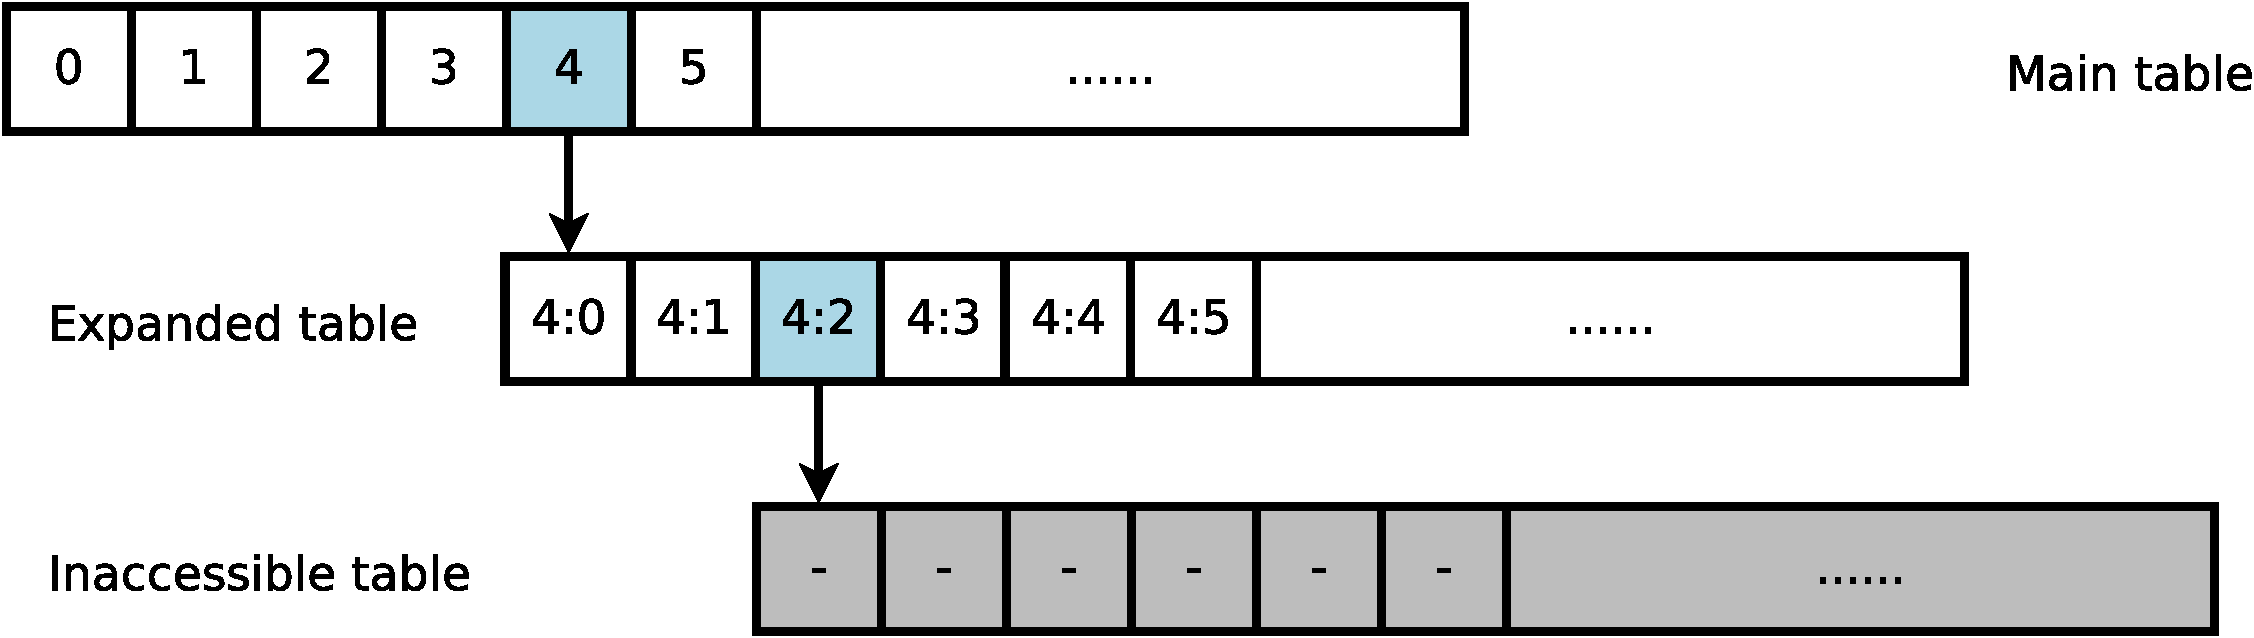
\includegraphics[width=0.72\textwidth]{Figure/image7.pdf}
    \caption{Capability Table Structure Diagram}
    \label{fig:2-3-capability-table-structure}
\end{figure}

\section{Capability Table Function List}\label{sec:2-capability-table-function-list}

The kernel functions related to capability tables are as follows:

\begin{xltabular}{\textwidth}{@{}>{\hsize=1.1605\hsize\raggedright\arraybackslash}X>{\hsize=0.8843\hsize\raggedright\arraybackslash}X>{\hsize=0.9552\hsize\raggedright\arraybackslash}X@{}}
\caption{Capability Table Related Kernel Functions}\label{tab:2-3-capability-table-kernel-functions}\\
\toprule
Call number & Type & Purpose\tabularnewline
\endfirsthead
\toprule
Call number & Type & Purpose\tabularnewline
\midrule
\endhead
\bottomrule
\endlastfoot
RME\_SVC\_CPT\_CRT & System call & Create a capability table\tabularnewline
RME\_SVC\_CPT\_DEL & System call & Delete a capability table\tabularnewline
RME\_SVC\_CPT\_ADD & System call & Capability delegation\tabularnewline
RME\_SVC\_CPT\_FRZ & System call & Capability freezing\tabularnewline
RME\_SVC\_CPT\_REM & System call & Capability removal\tabularnewline
\end{xltabular}
\nopagebreak[4]

The operation flags of capability table capabilities are as follows:

\begin{xltabular}{\textwidth}{@{}>{\hsize=0.9567\hsize\raggedright\arraybackslash}X>{\hsize=0.6339\hsize\raggedright\arraybackslash}X>{\hsize=1.4095\hsize\raggedright\arraybackslash}X@{}}
\caption{Capability Table Operation Flags}\label{tab:2-4-capability-table-operation-flags}\\
\toprule
Flag & Bit & Purpose\tabularnewline
\endfirsthead
\toprule
Flag & Bit & Purpose\tabularnewline
\midrule
\endhead
\bottomrule
\endlastfoot
RME\_CPT\_FLAG\_CRT & {[}0{]} &
Allow capabilities to be created in this capability table.\tabularnewline
RME\_CPT\_FLAG\_DEL & {[}1{]} &
Allow capabilities in this capability table to be deleted.\tabularnewline
RME\_CPT\_FLAG\_FRZ & {[}2{]} &
Allow capabilities in this capability table to be frozen.\tabularnewline
RME\_CPT\_FLAG\_ADD\_SRC & {[}3{]} &
Allow this capability table to serve as the source table in capability delegation.\tabularnewline
RME\_CPT\_FLAG\_ADD\_DST & {[}4{]} &
Allow this capability table to serve as the destination table in capability delegation.\tabularnewline
RME\_CPT\_FLAG\_REM & {[}5{]} &
Allow capabilities in this capability table to be removed.\tabularnewline
RME\_CPT\_FLAG\_PRC\_CRT & {[}6{]} &
Allow this capability table to be used as the process's capability table when creating a process.\tabularnewline
RME\_CPT\_FLAG\_PRC\_CPT & {[}7{]} &
Allow this capability table to replace the capability table of a process.\tabularnewline
\end{xltabular}
\nopagebreak[4]

For bit{[}6{]} and bit{[}7{]} in the table above, please refer to\ref{subsec:4-create-a-process}
and\ref{subsec:4-change-process-capability-table}
.

\subsection{Capability Table Creation}\label{subsec:2-create-a-capability-table}

This operation creates a capability table and places its capability into some existing capability table. A capability table is a kernel object, so the kernel memory it uses must be designated at creation time. In RME, we adopt the method of a kernel memory capability plus a kernel-relative start virtual address to determine the real kernel virtual address of the kernel object. Each kernel memory capability designates an allowed range\footnote{consisting of the kernel memory start absolute virtual address and the kernel memory end absolute virtual address}, and only kernel memory within this range can be used when creating kernel objects. The real kernel virtual address of the kernel object is the kernel start absolute virtual address of this kernel memory capability plus the kernel-relative start virtual address (Relative
Address,
Raddr) additionally designated when creating the kernel object. This point is the same for other kernel objects including capability tables, and will not be repeated in later chapters. For detailed information about kernel memory capabilities, please refer to\ref{sec:3-kernel-memory-function-list}
.

The capability table creation operation requires the following parameters:

\begin{xltabular}{\textwidth}{@{}>{\hsize=0.7639\hsize\raggedright\arraybackslash}X>{\hsize=0.6758\hsize\raggedright\arraybackslash}X>{\hsize=0.6758\hsize\raggedright\arraybackslash}X>{\hsize=1.8846\hsize\raggedright\arraybackslash}X@{}}
\caption{Parameters Required for Capability Table Creation}\label{tab:2-5-create-capability-table-parameters}\\
\toprule
Parameter name & Type & Field & Description\tabularnewline
\endfirsthead
\toprule
Parameter name & Type & Field & Description\tabularnewline
\midrule
\endhead
\bottomrule
\endlastfoot
Svc\_Num & ptr\_t & N & Must be RME\_SVC\_CPT\_CRT.\tabularnewline
Cap\_Cpt\_Crt & cid\_t & C &
A capability number corresponding to a capability table capability that must have the RME\_CPT\_FLAG\_CRT attribute; the capability corresponding to this capability number points to the capability table that is to receive this newly created capability table capability. This capability number can be a one-level or two-level lookup encoding.\tabularnewline
Cap\_Kom & cid\_t & P1.D1 &
A kernel memory capability number; the kernel memory range it identifies must be able to hold the entire capability table, and it must have the RME\_KOM\_FLAG\_CPT attribute. This capability number can be a one-level or two-level lookup encoding.\tabularnewline
Cap\_Crt & cid\_t & P1.D0 &
A capability number corresponding to some position of the capability table that is to receive this newly created capability table capability. The capability corresponding to this capability number must be empty. This capability number can only be a one-level lookup encoding.\tabularnewline
Raddr & ptr\_t & P2 &
The kernel-relative start virtual address to be used by the newly created capability table. This address is relative to the start virtual address of the kernel capability corresponding to Cap\_Kom.\tabularnewline
Entry\_Num & ptr\_t & P3 &
The number of entries contained in this capability table, which must be between 1 and RME\_CID\_2L. If RME\_CPT\_ENTRY\_MAX\footnote{see 7.3.2} is defined as a value that is less than RME\_CID\_2L and not 0, then this number must be between 1 and RME\_CPT\_ENTRY\_MAX.\tabularnewline
\end{xltabular}
\nopagebreak[4]

\needspace{16\baselineskip}
The return values of this operation may be as follows:

\begin{xltabular}{\textwidth}{@{}>{\hsize=0.7950\hsize\raggedright\arraybackslash}X>{\hsize=1.2050\hsize\raggedright\arraybackslash}X@{}}
\caption{Possible Return Values for Capability Table Creation}\label{tab:2-6-create-capability-table-return-values}\\
\toprule
Return value & Meaning\tabularnewline
\endfirsthead
\toprule
Return value & Meaning\tabularnewline
\midrule
\endhead
\bottomrule
\endlastfoot
    0 & The operation succeeded.\tabularnewline
    RME\_ERR\_CPT\_RANGE & The passed parameter for the number of capability table capabilities is outside the allowed range.\tabularnewline
    RME\_ERR\_CPT\_RANGE & The one-level/two-level lookup of Cap\_Cpt\_Crt is out of range.\tabularnewline
    RME\_ERR\_CPT\_RANGE & The one-level/two-level lookup of Cap\_Kom is out of range.\tabularnewline
    RME\_ERR\_CPT\_RANGE & The one-level lookup of Cap\_Crt is out of range.\tabularnewline
    RME\_ERR\_CPT\_FROZEN & The capability of the one-level/two-level lookup of Cap\_Cpt\_Crt has already been frozen.\tabularnewline
    RME\_ERR\_CPT\_FROZEN & The capability of the one-level/two-level lookup of Cap\_Kom has already been frozen.\tabularnewline
    RME\_ERR\_CPT\_FROZEN & Cap\_Crt is frozen, or another core is creating a capability at that position.\tabularnewline
    RME\_ERR\_CPT\_TYPE & Cap\_Cpt\_Crt is not a capability table capability.\tabularnewline
    RME\_ERR\_CPT\_TYPE & Cap\_Kom is not a kernel memory capability.\tabularnewline
    RME\_ERR\_CPT\_FLAG & Cap\_Cpt\_Crt does not have the RME\_CPT\_FLAG\_CRT attribute.\tabularnewline
    RME\_ERR\_CPT\_FLAG & Cap\_Kom does not have the RME\_KOM\_FLAG\_CPT attribute, or the range is incorrect.\tabularnewline
    RME\_ERR\_CPT\_EXIST & Cap\_Crt is not an empty capability.\tabularnewline
    RME\_ERR\_CPT\_KOT & Failed to allocate kernel memory.\tabularnewline
\end{xltabular}
\nopagebreak[4]

\subsection{Capability Table Deletion}\label{subsec:2-delete-a-capability-table}

This operation deletes a capability table. The capability table being deleted must not contain capabilities; that is, all of its capability positions should be empty. Deleting a capability table requires the following parameters:

\begin{xltabular}{\textwidth}{@{}>{\hsize=0.7639\hsize\raggedright\arraybackslash}X>{\hsize=0.6758\hsize\raggedright\arraybackslash}X>{\hsize=0.6758\hsize\raggedright\arraybackslash}X>{\hsize=1.8846\hsize\raggedright\arraybackslash}X@{}}
\caption{Parameters Required for Capability Table Deletion}\label{tab:2-7-delete-capability-table-parameters}\\
\toprule
Parameter name & Type & Field & Description\tabularnewline
\endfirsthead
\toprule
Parameter name & Type & Field & Description\tabularnewline
\midrule
\endhead
\bottomrule
\endlastfoot
Svc\_Num & ptr\_t & N & Must be RME\_SVC\_CPT\_DEL.\tabularnewline
Cap\_Cpt\_Del & cid\_t & C &
A capability number corresponding to a capability table capability that must have the RME\_CPT\_FLAG\_DEL attribute; the capability corresponding to this capability number points to the capability table that contains the capability table capability being deleted. This capability number can be a one-level or two-level lookup encoding.\tabularnewline
Cap\_Del & cid\_t & P1 &
A capability number corresponding to the capability table capability that is to be deleted. The capability corresponding to this capability number must be a capability table capability. This capability number can only be a one-level lookup encoding.\tabularnewline
\end{xltabular}
\nopagebreak[4]

The return values of this operation may be as follows:

\begin{xltabular}{\textwidth}{@{}>{\hsize=0.7450\hsize\raggedright\arraybackslash}X>{\hsize=1.2550\hsize\raggedright\arraybackslash}X@{}}
\caption{Possible Return Values for Capability Table Deletion}\label{tab:2-8-delete-capability-table-return-values}\\
\toprule
Return value & Meaning\tabularnewline
\endfirsthead
\toprule
Return value & Meaning\tabularnewline
\midrule
\endhead
\bottomrule
\endlastfoot
    0 & The operation succeeded.\tabularnewline
    RME\_ERR\_CPT\_RANGE & The one-level/two-level lookup of Cap\_Cpt\_Del is out of range.\tabularnewline
    RME\_ERR\_CPT\_RANGE & The one-level lookup of Cap\_Del is out of range.\tabularnewline
    RME\_ERR\_CPT\_FROZEN & The capability of the one-level/two-level lookup of Cap\_Cpt\_Del has already been frozen.\tabularnewline
    RME\_ERR\_CPT\_FROZEN & Cap\_Del has not been frozen.\tabularnewline
    RME\_ERR\_CPT\_TYPE & Cap\_Cpt\_Del is not a capability table capability.\tabularnewline
    RME\_ERR\_CPT\_TYPE & Cap\_Del is not a capability table capability.\tabularnewline
    RME\_ERR\_CPT\_NULL & Cap\_Del is an empty capability.\tabularnewline
    RME\_ERR\_CPT\_NULL & Two cores simultaneously try to delete this capability table; the core that does not succeed returns this value.\tabularnewline
    RME\_ERR\_CPT\_FLAG & Cap\_Cpt\_Del does not have the RME\_CPT\_FLAG\_DEL attribute.\tabularnewline
    RME\_ERR\_CPT\_QUIE & Cap\_Del is not quiescent.\tabularnewline
    RME\_ERR\_CPT\_EXIST & The capability table corresponding to Cap\_Del still contains capabilities.\tabularnewline
    RME\_ERR\_CPT\_REFCNT & The reference count of Cap\_Del is not 0, or it is not a root capability.\tabularnewline
\end{xltabular}
\nopagebreak[4]

\subsection{Capability Delegation}\label{subsec:2-transfer-a-capability}

This operation delegates a certain capability in one capability table into an empty position of another capability table. The parent capability of the newly created destination capability is the source capability, and the reference count of the source capability is incremented by 1. Performing capability delegation between capability tables requires the following parameters:

\begin{xltabular}{\textwidth}{@{}>{\hsize=0.7639\hsize\raggedright\arraybackslash}X>{\hsize=0.6758\hsize\raggedright\arraybackslash}X>{\hsize=0.6758\hsize\raggedright\arraybackslash}X>{\hsize=1.8846\hsize\raggedright\arraybackslash}X@{}}
\caption{Parameters Required for Capability Delegation}\label{tab:2-9-capability-transfer-parameters}\\
\toprule
Parameter name & Type & Field & Description\tabularnewline
\endfirsthead
\toprule
Parameter name & Type & Field & Description\tabularnewline
\midrule
\endhead
\bottomrule
\endlastfoot
Svc\_Num & ptr\_t & N & Must be RME\_SVC\_CPT\_ADD.\tabularnewline
Cap\_Cpt\_Dst & cid\_t & P1.D1 &
A capability number corresponding to a capability table capability that must have the RME\_CPT\_FLAG\_ADD\_DST attribute; the capability corresponding to this capability number points to the destination capability table. This capability number can be a one-level or two-level lookup encoding.\tabularnewline
Cap\_Dst & cid\_t & P1.D0 &
A capability number corresponding to the position that will receive the delegated capability. The capability corresponding to this capability number must be empty. This capability number can only be a one-level lookup encoding.\tabularnewline
Cap\_Cpt\_Src & cid\_t & P2.D1 &
A capability number corresponding to a capability table capability that must have the RME\_CPT\_FLAG\_ADD\_SRC attribute; the capability corresponding to this capability number points to the source capability table. This capability number can be a one-level or two-level lookup encoding.\tabularnewline
Cap\_Src & cid\_t & P2.D0 &
A capability number corresponding to the capability to be delegated. The capability corresponding to this capability number must not be empty and must not be frozen. This capability number can only be a one-level lookup encoding.\tabularnewline
Flags & ptr\_t & P3 &
The operation flag attributes to be delegated. Only the operations permitted by this operation flag can be performed by the newly created capability.\tabularnewline
\end{xltabular}
\nopagebreak[4]

It is worth noting that for kernel memory capabilities, additional bits placed in the system call number N and the capability table capability number C are also required during delegation to help determine their operation flag attributes. For the specific parameter passing method, please refer to\ref{sec:3-kernel-memory-function-list}
.

The return values of this operation may be as follows:

\begin{xltabular}{\textwidth}{@{}>{\hsize=0.6791\hsize\raggedright\arraybackslash}X>{\hsize=1.3209\hsize\raggedright\arraybackslash}X@{}}
\caption{Possible Return Values for Capability Delegation}\label{tab:2-10-capability-transfer-return-values}\\
\toprule
Return value & Meaning\tabularnewline
\endfirsthead
\toprule
Return value & Meaning\tabularnewline
\midrule
\endhead
\bottomrule
\endlastfoot
    0 & The operation succeeded.\tabularnewline
    RME\_ERR\_CPT\_RANGE & The one-level/two-level lookup of Cap\_Cpt\_Dst or Cap\_Cpt\_Src is out of range.\tabularnewline
    RME\_ERR\_CPT\_RANGE & The one-level lookup of Cap\_Dst or Cap\_Src is out of range.\tabularnewline
    RME\_ERR\_CPT\_FROZEN & The capability of the one-level/two-level lookup of Cap\_Cpt\_Dst or Cap\_Cpt\_Src is frozen.\tabularnewline
    RME\_ERR\_CPT\_FROZEN & Cap\_Src is frozen.\tabularnewline
    RME\_ERR\_CPT\_TYPE & Cap\_Cpt\_Dst or Cap\_Cpt\_Src is not a capability table capability.\tabularnewline
    RME\_ERR\_CPT\_NULL & Cap\_Src is an empty capability.\tabularnewline
    RME\_ERR\_CPT\_FLAG & Cap\_Cpt\_Src does not have the RME\_CPT\_FLAG\_ADD\_SRC attribute.\tabularnewline
    RME\_ERR\_CPT\_FLAG & Cap\_Cpt\_Dst does not have the RME\_CPT\_FLAG\_ADD\_DST attribute.\tabularnewline
    RME\_ERR\_CPT\_FLAG & The operation flag attributes of Cap\_Src conflict with the passed operation flag attributes; that is, the passed attributes include operations or operation ranges that Cap\_Src does not permit.\tabularnewline
    RME\_ERR\_CPT\_FLAG & The passed operation flag attributes are invalid, for example the upper and lower bounds of the operation range conflict, or no operation at all is permitted on the capability produced by the delegation.\tabularnewline
    RME\_ERR\_CPT\_EXIST & Cap\_Dst is not an empty capability.\tabularnewline
    RME\_ERR\_CPT\_REFCNT & The reference count of Cap\_Src exceeds the maximum range allowed by the system. On 32-bit systems the upper limit is $2^{23}-1$, and on 64-bit systems the upper limit is $2^{46}-1$. This is usually sufficient.\tabularnewline
\end{xltabular}
\nopagebreak[4]

\needspace{30\baselineskip}
\subsection{Capability Freezing}\label{subsec:2-freeze-a-capability}
\nopagebreak[4]

This operation freezes a capability in a capability table. If a capability is frozen, then after the quiescence period it is guaranteed that all operations on the kernel object pointed to by this capability that are initiated from this capability have stopped in the kernel, and at this point the capability can be deleted or removed. Note that this is not equivalent to all operations on the kernel object pointed to by this capability having stopped, because there may also be other capabilities pointing to this kernel object, and kernel object operations initiated from these capabilities can still proceed. Only if the root capability is frozen is it guaranteed that all operations on this kernel object have stopped, and only then can this capability and the kernel object be deleted. The capability freezing operation is also performed atomically by a compare-and-swap operation; however, when it fails, we know that some other core must have successfully helped us freeze the capability, so success is still returned.

\needspace{20\baselineskip}
Freezing a capability requires the following parameters:

\begin{xltabular}{\textwidth}{@{}>{\hsize=0.7639\hsize\raggedright\arraybackslash}X>{\hsize=0.6758\hsize\raggedright\arraybackslash}X>{\hsize=0.6758\hsize\raggedright\arraybackslash}X>{\hsize=1.8846\hsize\raggedright\arraybackslash}X@{}}
\caption{Parameters Needed for Capability Freezing}\label{tab:2-11-capability-freeze-parameters}\\
\toprule
Parameter Name & Type & Domain & Description\tabularnewline
\endfirsthead
\toprule
Parameter Name & Type & Domain & Description\tabularnewline
\midrule
\endhead
\bottomrule
\endlastfoot
Svc\_Num & ptr\_t & N & Must be RME\_SVC\_CPT\_FRZ.\tabularnewline
Cap\_Cpt\_Frz & cid\_t & C &
A capability number corresponding to a capability table capability that must have the RME\_CPT\_FLAG\_FRZ attribute; the capability referenced by this capability number points to the capability table containing the capability being frozen. This capability number may be a one-level or two-level lookup encoding.\tabularnewline
Cap\_Frz & cid\_t & P1 &
A capability number corresponding to the capability to be frozen. This capability number can only be a one-level lookup encoding.\tabularnewline
\end{xltabular}
\nopagebreak[4]

The return values of this operation may be as follows:

\begin{xltabular}{\textwidth}{@{}>{\hsize=0.7950\hsize\raggedright\arraybackslash}X>{\hsize=1.2050\hsize\raggedright\arraybackslash}X@{}}
\caption{Possible Return Values for Capability Freezing}\label{tab:2-12-capability-freeze-return-values}\\
\toprule
Return Value & Meaning\tabularnewline
\endfirsthead
\toprule
Return Value & Meaning\tabularnewline
\midrule
\endhead
\bottomrule
\endlastfoot
    0 & The operation succeeded.\tabularnewline
    RME\_ERR\_CPT\_RANGE & The one-level/two-level lookup of Cap\_Cpt\_Frz is out of range.\tabularnewline
    RME\_ERR\_CPT\_RANGE & The one-level lookup of Cap\_Frz is out of range.\tabularnewline
    RME\_ERR\_CPT\_FROZEN & The capability found by the one-level/two-level lookup of Cap\_Cpt\_Frz is already frozen.\tabularnewline
    RME\_ERR\_CPT\_FROZEN & Cap\_Frz is already frozen and does not need to be frozen again, or it is being created.\tabularnewline
    RME\_ERR\_CPT\_TYPE & Cap\_Cpt\_Frz is not a capability table capability.\tabularnewline
    RME\_ERR\_CPT\_NULL & Cap\_Frz is an empty capability.\tabularnewline
    RME\_ERR\_CPT\_FLAG & Cap\_Cpt\_Frz does not have the RME\_CPT\_FLAG\_FRZ attribute.\tabularnewline
    RME\_ERR\_CPT\_QUIE & Cap\_Frz is not quiescent.\tabularnewline
    RME\_ERR\_CPT\_REFCNT & The reference count of Cap\_Frz is not 0.\tabularnewline
\end{xltabular}
\nopagebreak[4]

\subsection{Capability Removal}\label{subsec:2-remove-a-capability}

This operation removes a capability from a capability table. The capability being removed must not be a root capability\footnote{The deletion operation should be used for root capabilities}. Removing a capability does not cause the kernel object associated with it to be removed; only the capability itself is removed\footnote{The deletion operation, by contrast, can only be used on a root capability that is not referenced, and it deletes both the root capability and the kernel object at the same time}. The capability removal operation is also performed atomically by a compare-and-swap operation; however, when it fails, we know that some other core must have successfully helped us remove the capability, so success is still returned.

\needspace{20\baselineskip}
Removing a capability requires the following parameters:

\begin{xltabular}{\textwidth}{@{}>{\hsize=0.7639\hsize\raggedright\arraybackslash}X>{\hsize=0.6758\hsize\raggedright\arraybackslash}X>{\hsize=0.6758\hsize\raggedright\arraybackslash}X>{\hsize=1.8846\hsize\raggedright\arraybackslash}X@{}}
\caption{Parameters Needed for Capability Removal}\label{tab:2-13-capability-removal-parameters}\\
\toprule
Parameter Name & Type & Domain & Description\tabularnewline
\endfirsthead
\toprule
Parameter Name & Type & Domain & Description\tabularnewline
\midrule
\endhead
\bottomrule
\endlastfoot
Svc\_Num & ptr\_t & N & Must be RME\_SVC\_CPT\_REM.\tabularnewline
Cap\_Cpt\_Rem & cid\_t & C &
A capability number corresponding to a capability table capability that must have the RME\_CPT\_FLAG\_REM attribute; the capability referenced by this capability number points to the capability table containing the capability being removed. This capability number may be a one-level or two-level lookup encoding.\tabularnewline
Cap\_Rem & cid\_t & P1 &
A capability number corresponding to the capability to be removed. This capability number can only be a one-level lookup encoding.\tabularnewline
\end{xltabular}
\nopagebreak[4]

The return values of this operation may be as follows:

\begin{xltabular}{\textwidth}{@{}>{\hsize=0.7554\hsize\raggedright\arraybackslash}X>{\hsize=1.2446\hsize\raggedright\arraybackslash}X@{}}
\caption{Possible Return Values for Capability Removal}\label{tab:2-14-capability-removal-return-values}\\
\toprule
Return Value & Meaning\tabularnewline
\endfirsthead
\toprule
Return Value & Meaning\tabularnewline
\midrule
\endhead
\bottomrule
\endlastfoot
    0 & The operation succeeded.\tabularnewline
    RME\_ERR\_CPT\_RANGE & The one-level/two-level lookup of Cap\_Cpt\_Rem is out of range.\tabularnewline
    RME\_ERR\_CPT\_RANGE & The one-level lookup of Cap\_Rem is out of range.\tabularnewline
    RME\_ERR\_CPT\_FROZEN & The capability found by the one-level/two-level lookup of Cap\_Cpt\_Rem is already frozen.\tabularnewline
    RME\_ERR\_CPT\_FROZEN & Cap\_Rem is not frozen.\tabularnewline
    RME\_ERR\_CPT\_TYPE & Cap\_Cpt\_Rem is not a capability table capability.\tabularnewline
    RME\_ERR\_CPT\_NULL & Cap\_Rem is an empty capability.\tabularnewline
    RME\_ERR\_CPT\_NULL & Two cores attempt to remove this capability simultaneously; in this case the core that did not succeed returns this value.\tabularnewline
    RME\_ERR\_CPT\_FLAG & Cap\_Cpt\_Rem does not have the RME\_CPT\_FLAG\_REM attribute.\tabularnewline
    RME\_ERR\_CPT\_QUIE & Cap\_Rem is not quiescent.\tabularnewline
    RME\_ERR\_CPT\_ROOT & Cap\_Rem is a root capability and cannot be removed; please use the deletion operation.\tabularnewline
\end{xltabular}
\nopagebreak[4]

\section{Bibliography of This Chapter}\label{sec:2-chapter-bibliography}

\protect\phantomsection\label{cite:2-1}

\noindent {[}1{]} J. B. Dennis and E. C. Van Horn, ``Programming semantics for multiprogrammed computations,'' \textit{Communications of the ACM}, vol. 9, pp. 143--155, 1966.

\protect\phantomsection\label{cite:2-2}

\noindent {[}2{]} J. S. Shapiro, J. M. Smith, and D. J. Farber, \textit{EROS: A Fast Capability System}, vol. 33. ACM, 1999.

\protect\phantomsection\label{cite:2-3}

\noindent {[}3{]} R. J. Feiertag and P. G. Neumann, ``The foundations of a provably secure operating system (PSOS),'' in \textit{Proceedings of the National Computer Conference}, 1979, pp. 329--334.

\protect\phantomsection\label{cite:2-4}

\noindent {[}4{]} Q. Wang, Y. Ren, M. Scaperoth, and G. Parmer, ``Speck: a kernel for scalable predictability,'' in \textit{Proceedings of the IEEE Real-Time and Embedded Technology and Applications Symposium (RTAS)}, 2015, pp. 121--132.

\protect\phantomsection\label{cite:2-5}

\noindent {[}5{]} G. Klein, K. Elphinstone, G. Heiser, J. Andronick, D. Cock, P. Derrin, et al., ``seL4: formal verification of an OS kernel,'' in \textit{Proceedings of the ACM SIGOPS 22nd Symposium on Operating Systems Principles}, Big Sky, MT, USA, 2009.

\protect\phantomsection\label{cite:2-6}

\noindent {[}6{]} B. W. Lampson, ``Protection,'' \textit{ACM SIGOPS Operating Systems Review}, vol. 8, pp. 18--24, 1974.

